\documentclass[11pt,a4paper,oneside]{article}

%\usepackage{pscyr}
\usepackage[T2A]{fontenc}
\usepackage[utf8x]{inputenc}
\usepackage[english,russian]{babel}
\usepackage{expdlist}
\usepackage[dvips]{graphicx}
\usepackage{subcaption}
\usepackage{amsmath}
\usepackage[makeroom]{cancel}
\usepackage{svg}
\usepackage[top=1in, bottom=1in, left=1in, right=1in]{geometry}
\usepackage{indentfirst}
\usepackage{mathtools}

\begin{document}

\begin{center}
	{Вяцков Михаил, КН-401}
	
	{\huge \bf Лабораторная работа №5}
\end{center}

\section{Условия}

Решить следующую задачу Коши на отрезке $[0, 1]$

$$ y' = f(x, y) = -5 y \cos(5 x) + 25 \sin(10 x), y(0) = 0 $$
$$ f'_y(x, y) = -5 \cos(5 x) $$

Заметим, что $\cos(x)$ и $\sin(x)$ арифметические функции, а значит бесконечное число раз дифференцируемы  по $x$ вместе с $f(x, y)$. Кроме того, $f(x, y)$ растет сублинейно, т.е. $\left| f(x, y) \right| \le m(x) (1 + |y|)$, где $m(x)$~--- некоторая дифференцируемая функция. Также, будучи линейной по $y$, $f(x, y)$ очевидно удовлетворяет условию липшицевости.

Таким образом можно заключить, что существует и притом единственное глобальное решение данного дифференциального уравнения $y(x)$.

\section{Методы}

\subsection{Эйлера с пересчетом}

Метод Эйлера с пересчетом на самом деле является методом Рунге-Кутты 2 порядка. Доказывается, что невязка метода имеет 3 порядок, а так как это явный метод РК, то значит сам метод сходится со вторым порядком.

Для подсчета очередного шага используется формула

$$ y_{n + 1} = y_n + \frac{h}{2} \left( f(x_n, y_n) + f(x_n + h, y_n + h f(x_n, y_n)) \right) $$

\subsection{Эйлера неявный}

Неяный метод Эйлера~--- частный случай неявного метода Адама (0 порядка). Построив интерполяционный многочлен и посчитав интеграл, получаем формулу

$$ y_{n + 1} = y_n + h f(x_{n + 1}, y_{n + 1}) $$

Данное нелинейное уравнение можно решить например с помощью метода Ньютона, который заключается в нахождении корня итерационным процессом вида

$$ g(z) = z - y_n - h f(x_{n + 1}, z) $$
$$ z_{l + 1} = z_{l} - \frac{g(z_l)}{g'(z_l)} $$

Начальное приближение можно сделать например методом Эйлера с пересчетом

$$ z_0 = y_n + \frac{h}{2} \left( f(x_n, y_n) + f(x_n + h, y_n + h f(x_n, y_n)) \right)$$

\pagebreak
\subsection{Рунге-Кутты 3 порядка}

Среди всего семейства методов Рунге-Куты 3 поряда возьмем

$$ y_{n + 1} = y_n + \frac{1}{6} k_1
	+ \frac{1}{6} k_2
	+ \frac{4}{6} k_3 $$
$$ k_1 = h f(x_n, y_n) $$
$$ k_2 = h f(x_n + h, y_n + k_1) $$
$$ k_3 = h f(x_n + \frac{h}{2}, y_n + \frac{1}{4} k_1 + \frac{1}{4} k_2) $$

Он сходится с третим порядком точности

\section{Численный эксперимент}

\begin{figure}[h]
	\begin{subfigure}{0.5\textwidth}
		\centering
		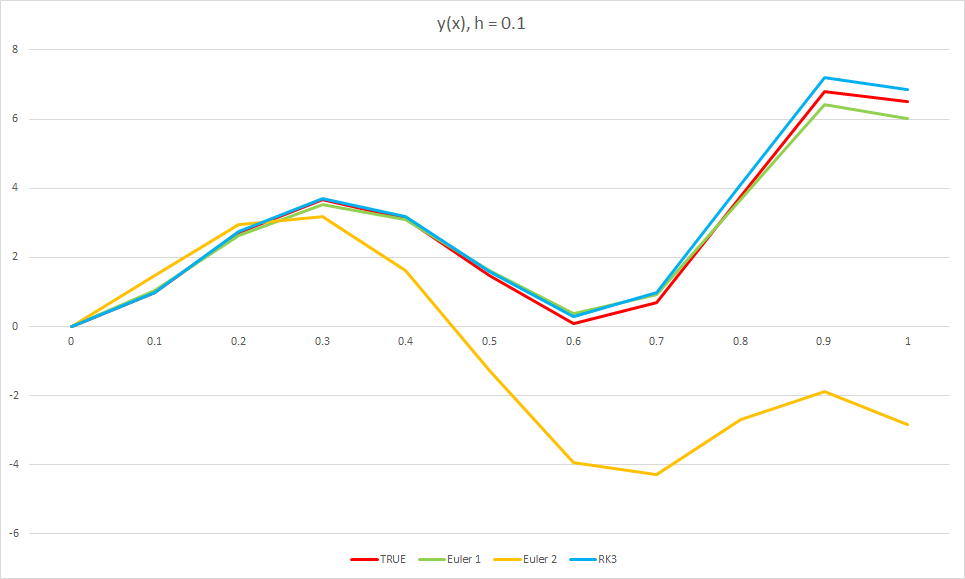
\includegraphics[width=0.9\linewidth]{pics/plot1.png}
		\caption{Шаг $h=0.1$}
	\end{subfigure}
	\begin{subfigure}{0.5\textwidth}
		\centering
		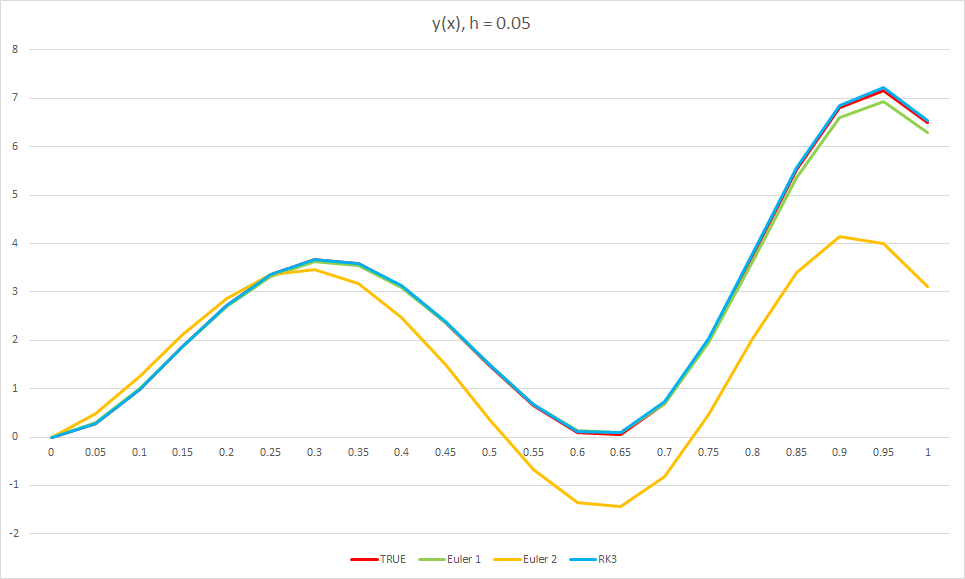
\includegraphics[width=0.9\linewidth]{pics/plot2.png}
		\caption{Шаг $h=0.05$}
	\end{subfigure}
	\begin{subfigure}{0.5\textwidth}
		\centering
		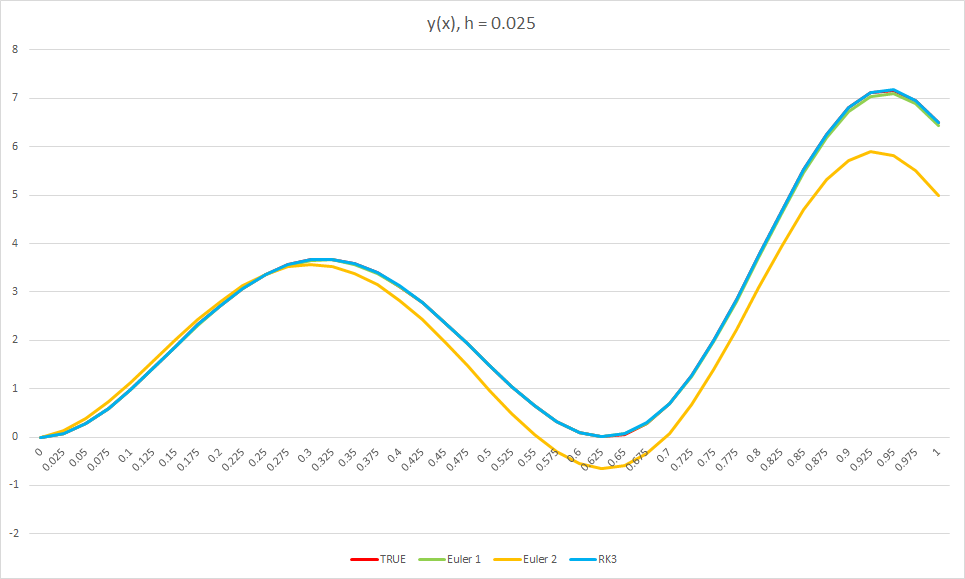
\includegraphics[width=0.9\linewidth]{pics/plot3.png}
		\caption{Шаг $h=0.025$}
	\end{subfigure}
	\begin{subfigure}{0.5\textwidth}
		\centering
		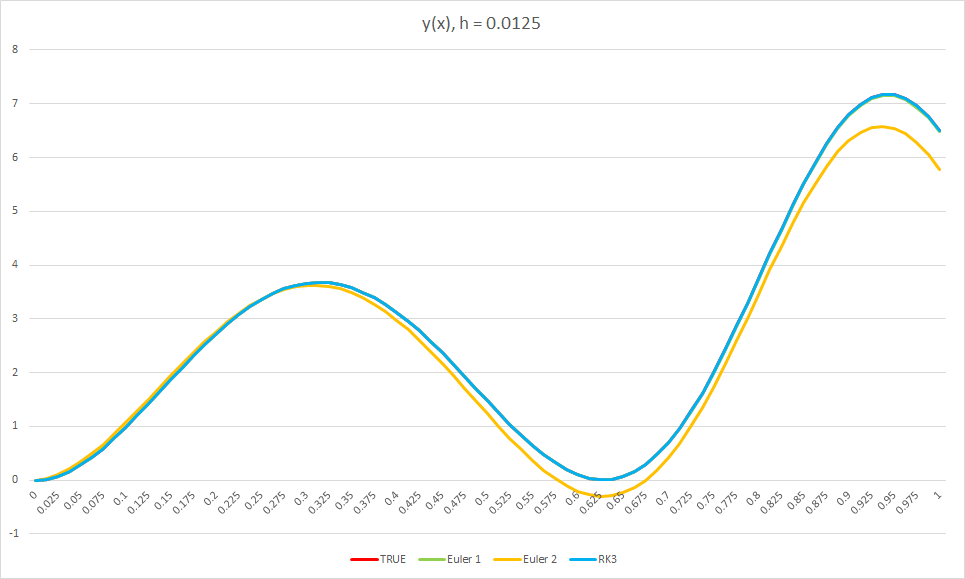
\includegraphics[width=0.9\linewidth]{pics/plot4.png}
		\caption{Шаг $h=0.0125$}
	\end{subfigure}
	\caption{Графики численного решение задачи Коши}
\end{figure}

\begin{figure}[h]
	\begin{subfigure}{\textwidth}
		\centering
		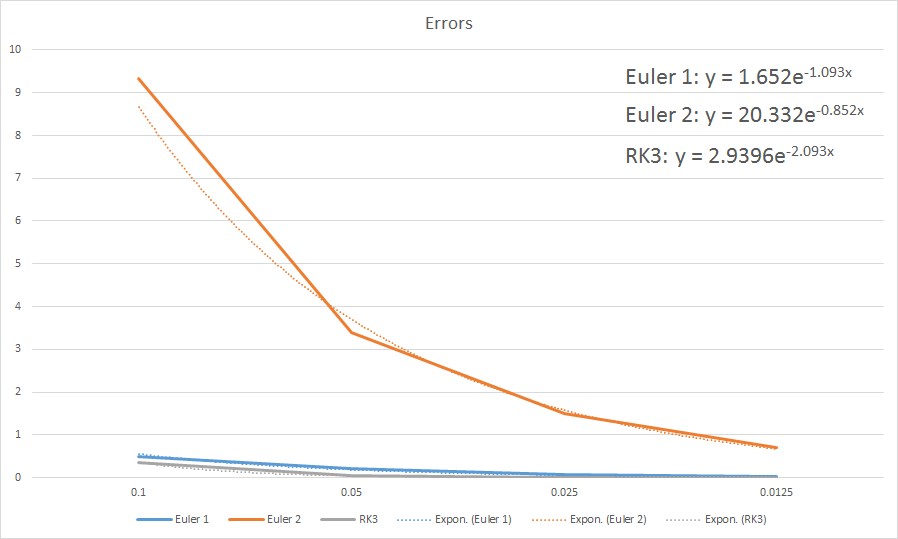
\includegraphics[width=0.9\linewidth]{pics/errors.png}
	\end{subfigure}
	\caption{График зависимости ошибки от размера шага}
\end{figure}

\section{Выводы}

Как и ожидалось, метод с наилучшим порядком точности (Рунге-Куты 3 порядка) оказался точнее всех, метод с наихудшим порядком точности (неявный метод Эйлера) оказался наименее точный, заметно отстав от остальных методов в точности. Кроме того, решение, построеное неявным методом Эйлера лишилось свойсва неотрицательности.

Рост ошибки на практике неплохо сошелся с теоретическими ожиданиями, так $e^{-0.852} \approx 0.43 \approx \frac{1}{2}$, $e^{-1.093} \approx 0.33 \approx \frac{1}{4}$ (скорее всего тут ошибка возникла при построении trendlin'а, из-за того, что первое решение оказалось точнее, чем оценивалось, это заметно даже зрительно, первый отрезок более пологий, чем экспонента), $e^{-2.093} \approx 0.123 \approx \frac{1}{8}$. Таким образом при экспоненциальном падении размера шага ошибка падала практически как ожидалось.

\end{document}
